%%%%%%%%%%%%%%%%%%%%%%%%%%%%%%%%%%%%%%%%%
% Beamer Presentation
% LaTeX Template
% Version 1.0 (10/11/12)
%
% This template has been downloaded from:
% http://www.LaTeXTemplates.com
%
% License:
% CC BY-NC-SA 3.0 (http://creativecommons.org/licenses/by-nc-sa/3.0/)
%
%%%%%%%%%%%%%%%%%%%%%%%%%%%%%%%%%%%%%%%%%

%----------------------------------------------------------------------------------------
%	PACKAGES AND THEMES
%----------------------------------------------------------------------------------------

\documentclass[usenames,dvipsnames,table]{beamer}

\mode<presentation> {

\usetheme{Madrid}
%\setbeamertemplate{footline} % To remove the footer line in all slides uncomment this line
%\setbeamertemplate{footline}[page number] % To replace the footer line in all slides with a simple slide count uncomment this line
\setbeamertemplate{navigation symbols}{} % To remove the navigation symbols from the bottom of all slides uncomment this line
}

\usepackage{graphicx} % Allows including images
\usepackage{booktabs} % Allows the use of \toprule, \midrule and \bottomrule in tables
\usepackage{listings}
\usepackage{xcolor}
\usepackage{xfrac}
% \usepackage{enumitem}

%----------------------------------------------------------------------------------------
%	TITLE PAGE
%----------------------------------------------------------------------------------------

\title[ABDA Ch 9]{Applied Bayesian Data Analysis --- Chapter 9}

\author{Kim Albertsson} % Your name
\institute[LTU and CERN]
{
CERN and Luleå University of Technology \\
\medskip
\textit{kim.albertsson@ltu.se}
}
\date{\today}

\newcommand{\cgy}{\cellcolor{gray!25}}
\newcommand{\cgr}{\cellcolor{green!25}}
\newcommand{\cye}{\cellcolor{orange!25}}
\newcommand{\ccb}{\cellcolor{Cerulean!25}}

\begin{document}

\begin{frame}
\titlepage % Print the title page as the first slide
\end{frame}

% \begin{frame}
% \frametitle{}
% \begin{itemize}
% \item
% \end{itemize}
% \end{frame}

%----------------------------------------------------------------------------------------
%	PRESENTATION SLIDES
%----------------------------------------------------------------------------------------
\section{Chapter 9}
\begin{frame}
\begin{center}
{\huge{Chapter 9}}
\\\vspace{2em}
Hierarchical models:\\
When parameters depend upon parameters

\vspace{5em}
{\small\textbf{Caveat:} Minimal coverage of JAGS.}
\end{center}
\end{frame}

\begin{frame}
\frametitle{Personal reflections}
\begin{itemize}
\item Hierarchical models: neat technique to lend statistical strength to model. Like priors, it seems an artform, as opposed to rigorous science. \textcolor{gray}{Not saying science cannot be done, just that it's ``softer''.}

\item Good examples to give one experience to lean back on. Explains intuitions behind and interpretations of distributions and paramters. E.g. mode of the beta distribution used as group mode (with physical interpretation).

\item Advice for double checking resutls helpful. E.g. checking priors.

\item Weak discussion on meaningful differences between predictions. So far only ``HDI interval covers null hypotesis'' therefore no difference between groups. \textcolor{gray}{Unsure if I use ``null hypothesis'' correctly here.}
\end{itemize}

\vspace{3em}
\begin{center}
\small%
Trick --- useful insight applicable once;\\
Technique --- insight with repeated, general, usefulness.
\end{center}
\end{frame}

\begin{frame}
\frametitle{Introduction}
Hierarchical models arise in many situations
\begin{itemize}
\item E.g. patient recovery after surgery. (Team success rate ($\theta_s$) depends on $\omega$, recovery rate for hospital.)
\item E.g. student buying lunch. (Child prob. of buying ($\theta_s$) depends on $\omega$, typical buy rate for school.)
\end{itemize}

Hierarchical refactoring:
\begin{align*}
p(\theta, \omega|D) \propto& p(D|\theta, \omega)p(\theta, \omega)\\
                          =& p(D|\theta) p(\theta|\omega)p(\omega) \tag{9.1}
\end{align*}
Compare to Eq.~(5.3) applied to the joint parameter probability
\begin{align*}
p(\theta, \omega|D) \propto& p(D|\theta, \omega)p(\theta, \omega)\\
                          =& p(D|\theta\textcolor{red}{, \omega})p(\theta|\omega)p(\omega) \tag{Using 5.3}
\end{align*}
I.e. in hierarchical models, data is not dependent on \emph{hidden} parameters.
\end{frame}

\begin{frame}
\frametitle{Introduction}
Benefits of hierarchical models:
\begin{itemize}
\item Interpretability
\item Data efficiency
\item Sampling efficiency (e.g. Gibbs sampling depends upon conditionals)
\end{itemize}
\end{frame}

\begin{frame}
\frametitle{A single coin from a single mint}
\begin{columns}[c]
\column{.5\textwidth}
\small
Hierarchical coin model: Factory produces coins with a typical bias.

{\tiny%
\begin{align*}
\gamma_i \sim Bernoulli(\theta)\tag{9.2}\\
\theta \sim \beta(a_\theta, b_\theta)\tag{9.3}\\
\theta \sim \beta(\omega(\kappa-2)+1, (1-\omega)(\kappa-2)+1)\tag{9.4}\\
\omega \sim \beta(a_\omega, b_\omega)\tag{9.5}\\
\kappa = K
\end{align*}}
\noindent $\omega$ is both mode of $\beta$ and parameter of model. $\kappa$ is concentration of $\beta$. Figure: Graphical representation of eq. system.

{\tiny%
\begin{align*}
p(\theta, \omega|\gamma) =& \frac{p(\gamma|\theta, \omega)p(\theta, \omega)}
                                {p(\gamma)}\\
                         =& \frac{p(\gamma|\theta)p(\theta|\omega)p(\theta)}
                                {p(\gamma)}\tag{9.6}
\end{align*}}

From def.: $\gamma$ depends only on $\theta$. From Eq.~5.3: factor joint.

\column{.5\textwidth}
\begin{figure}
\centering
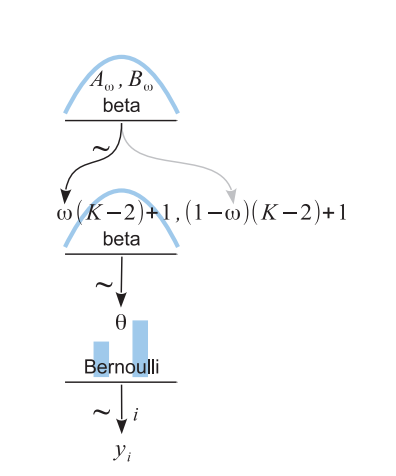
\includegraphics[width=\linewidth]{img/fig9_1}
\end{figure}
\end{columns}
\end{frame}

\begin{frame}
\frametitle{Aside: Hierarchy of data}
Given
\begin{align*}
\gamma_i \sim Bernoulli(\theta)\tag{9.2}\\
\theta \sim \beta(a, b)\tag{9.3}\\
p(\theta|\gamma) = p(\gamma|\theta)p(\theta)
\end{align*}
I.e. the posterior is factored into a chain of dependencies.

\vspace{1em}
Can we consider the system $\{\gamma, \theta\}$ a hierarchical model? Why; Why not? 
\end{frame}

\begin{frame}
\frametitle{Posterior through grid approximation (I)}
\begin{columns}[c]
\column{.5\textwidth}
Eq.~9.6 is difficult to solve analytically. Approximate with grid.

\vspace{1em}
Prior uses $b_\omega=2, b_\omega=2, K=100$. I.e. if we know $\omega$ we're fairly certain about $\theta$ (see $p(\theta|\omega=0.25)$ plot).

\vspace{1em}
Likelihood contours parallel, data depends only on $\theta$.

\vspace{1em}
Data mostly heads implies $\omega$ biased toward upper right quadrant due to tight coupling $\theta$, $\omega$.

\vspace{1em}
Note: Could use second coin to improve estimate of first!
\column{.5\textwidth}
\begin{figure}
\centering
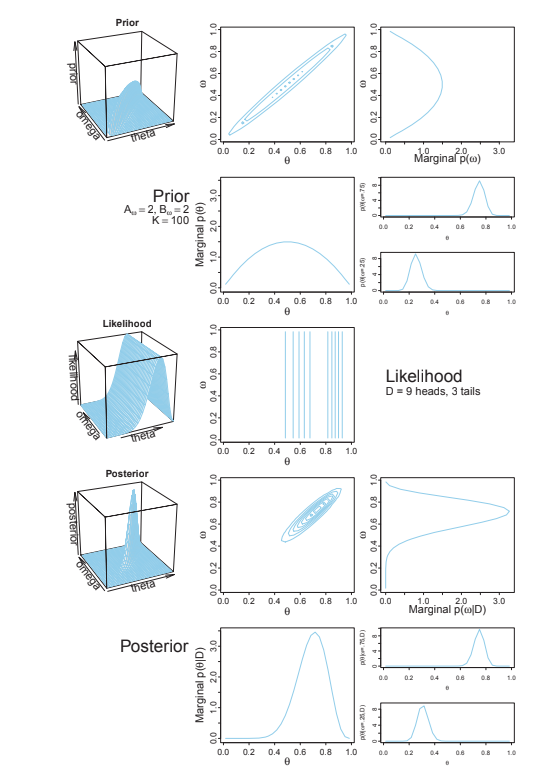
\includegraphics[height=0.8\textheight]{img/fig9_2}
\end{figure}
\end{columns}
\end{frame}

\begin{frame}
\frametitle{Posterior through grid approximation (II)}
\begin{columns}[c]
\column{.5\textwidth}
Prior uses $b_\omega=20, b_\omega=20, K=6$. I.e. $\omega$ certain but $\theta|\omega$ uncertain.

\vspace{1em}
Posterior mostly refines idea about $\theta$.

\vspace{1em}
Warning: Mismodelling? See posterior conditional plots. (Model supposes $\theta$ close to $\omega$.)
\column{.5\textwidth}
\begin{figure}
\centering
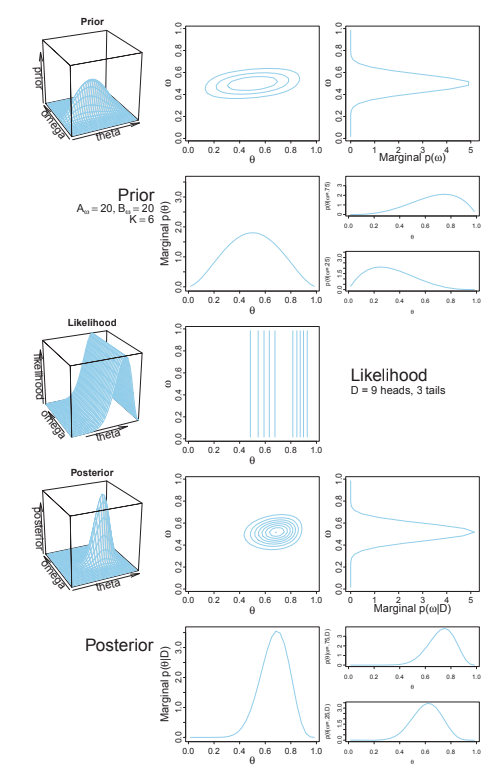
\includegraphics[height=0.8\textheight]{img/fig9_3}
\end{figure}
\end{columns}
\end{frame}

\begin{frame}
\frametitle{Multiple coins from single mint (I)}
\begin{columns}[c]
\column{.5\textwidth}
Typical case: E.g. testing memory after taking new drug (Note: Acutal variable of interest is the hidden one).

\vspace{1em}
Same as previous figure, with multiple $\theta$s.

\column{.5\textwidth}
\begin{figure}
\centering
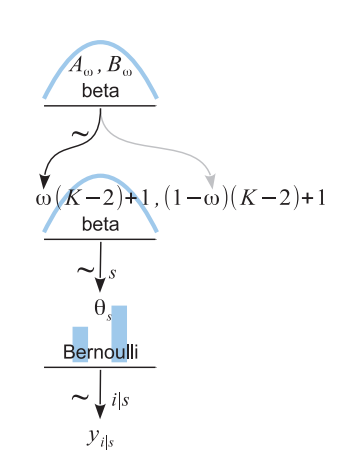
\includegraphics[height=0.8\textheight]{img/fig9_4}
\end{figure}
\end{columns}
\end{frame}

\begin{frame}
\frametitle{Multiple coins from single mint (II)}
\begin{columns}[c]
\column{.5\textwidth}
Weak coupling between coins ($K=5$).

{\tiny%
\begin{align*}
p(\theta_1, \theta_2, \omega|D) =& \frac{\textcolor{MidnightBlue}{p(D|\theta_1, \theta_2, \omega)}
                                         \textcolor{BurntOrange}{p(\theta_1, \theta_2, \omega)}}
                                       {p(D)}\\
                                =& \frac{\textcolor{MidnightBlue}{p(D_1|\theta_1)p(D_2|\theta_2)}
                                         \textcolor{BurntOrange}{p(\theta_1|\omega)p(\theta_2|\omega)p(\omega)}}
                                       {p(D)}
\end{align*}}

\vspace{1em}
(Not shown) Conditionals ($p(\theta_s|\omega)$) are spread out.

\vspace{1em}
Datasets imply spread in coin bias. Does little for $\omega$.

\column{.5\textwidth}
\begin{figure}
\centering
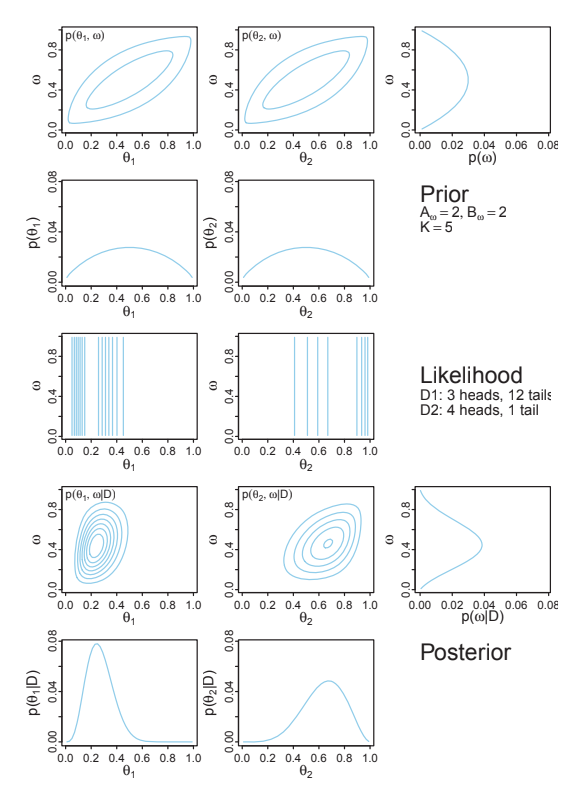
\includegraphics[height=0.8\textheight]{img/fig9_5}
\end{figure}
\end{columns}
\end{frame}

\begin{frame}
\frametitle{Multiple coins from single mint (III)}
\begin{columns}[c]
\column{.5\textwidth}
Strong coupling between coins ($K=75$).

\vspace{1em}
(Not shown) Conditionals ($p(\theta_s|\omega)$) are concentrated.

\vspace{1em}
Datasets are contradictory (with strong coupling). Data from larger set dominates. Constrains $\omega$.

\vspace{1em}
Grid approximation only feasible in low dimensions.
\column{.5\textwidth}
\begin{figure}
\centering
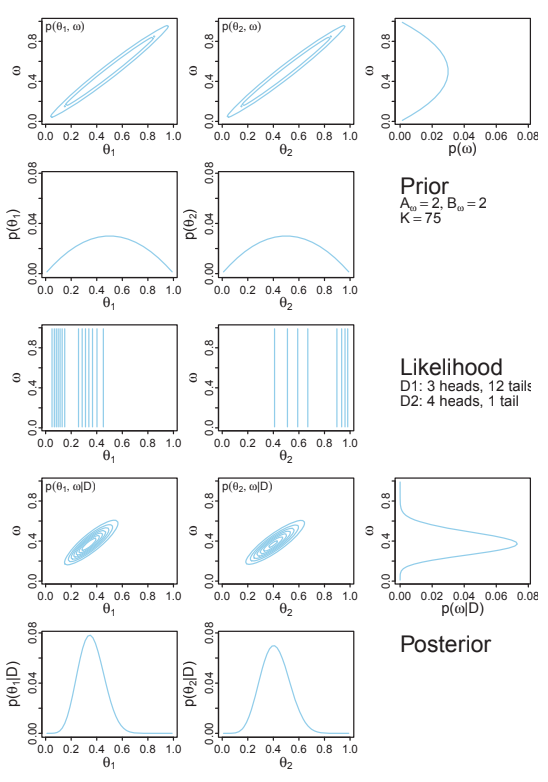
\includegraphics[height=0.8\textheight]{img/fig9_6}
\end{figure}
\end{columns}
\end{frame}

\begin{frame}
\frametitle{Gamma distribution}
\footnotesize
Generalised exponential distribution much like $\beta$ is generalised uniform (among others).
\begin{columns}[c]
\column{.5\textwidth}
\begin{align*}
\mathrm{Gamma}(\kappa|s, r=\theta^{-1});& \mathrm{\ where\ } s \mathrm{:\ shape,\ }r\mathrm{:\ rate}
\end{align*}

{\tiny%
\begin{align*}
s=\frac{\mu^2}{\sigma^2};\ r=\frac{\mu}{\sigma^2};\ \mu>0 \tag{9.7} \mathrm{\ (mean)} \\
s=1+\omega r;\ r=\frac{\omega\sqrt{\omega^2+4\sigma^2}}{2\sigma^2};\ \omega>0 \mathrm{\ (mode)} \tag{9.8}
\end{align*}}

Related distributions:
\begin{itemize}
\item Exponential distribution $\exp(\lambda)=\mathrm{Gamma}(1, \lambda^{-1})$, models e.g. random decay of particles or electronical components. 
\item Chi-square $\chi^2(k)=\mathrm{Gamma}(k/2, 2)$, models sum of $k$ independent standard normal random variables.
\item ... and many more ...
\end{itemize}

\column{.5\textwidth}
\begin{figure}
\centering
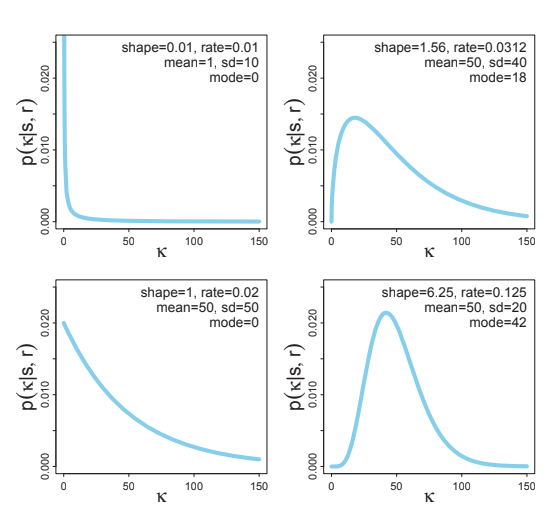
\includegraphics[width=\linewidth]{img/fig9_8}
\end{figure}
\end{columns}
\end{frame}

\begin{frame}
\frametitle{A realistic model with MCMC}
\begin{columns}[c]
\column{.5\textwidth}
Add realism by
\begin{itemize}
\item Relax constraint on $\kappa$ (draw from Gamma).
\item More subjects/coins!
\end{itemize}
Intuitively, for each coin, $\kappa$ small: data clustered. If $\kappa$ large: data spread out. 
\column{.5\textwidth}
\begin{figure}
\centering
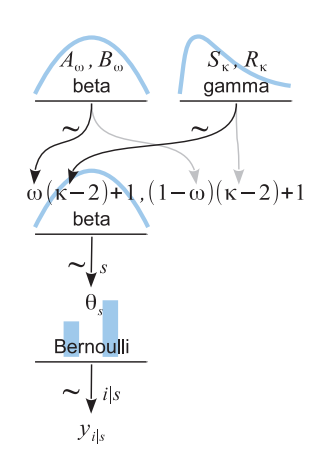
\includegraphics[width=\linewidth]{img/fig9_7}
\end{figure}
\end{columns}
\end{frame}

\begin{frame}
\frametitle{Therapeutic touch (I)}
\begin{columns}[c]
\column{.5\textwidth}
Recreate investigation of Rosa et al. (1998): Can practitioners feel a body's energy field?

\begin{itemize}
\item Flip coin and place experimenter hand near practitioner hand.
\item Practitioner reports which hand is closest (binary classification).
\item 28 subjects (with caveat)
\item Skill of each practitioner: $\theta_s$.
\item Effect in group: $\omega$.
\item Data in Figure.
\end{itemize}
\column{.5\textwidth}
\begin{figure}
\centering
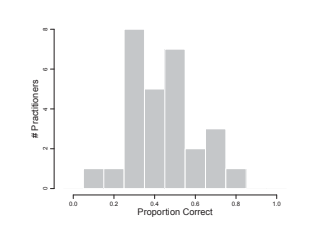
\includegraphics[width=\linewidth]{img/fig9_9}
\end{figure}
\end{columns}
\end{frame}

\begin{frame}
\frametitle{Therapeutic touch (II)}
\begin{columns}[c]
\column{.5\textwidth}
$\kappa$ shows high auto-correlation (common for chains for high-level parameters). Accuracy of $\kappa$ not a concern (Why: small changes in \kappa does induces only small change in other variables).

\vspace{1em}
Practitioners, as a class: No effect.

\vspace{1em}
Plus shows score of individual. Deviates from mode due to hierarchical modelling.

\vspace{1em}
Differences: Do subjects perform differently? No!

\column{.5\textwidth}
\begin{figure}
\centering
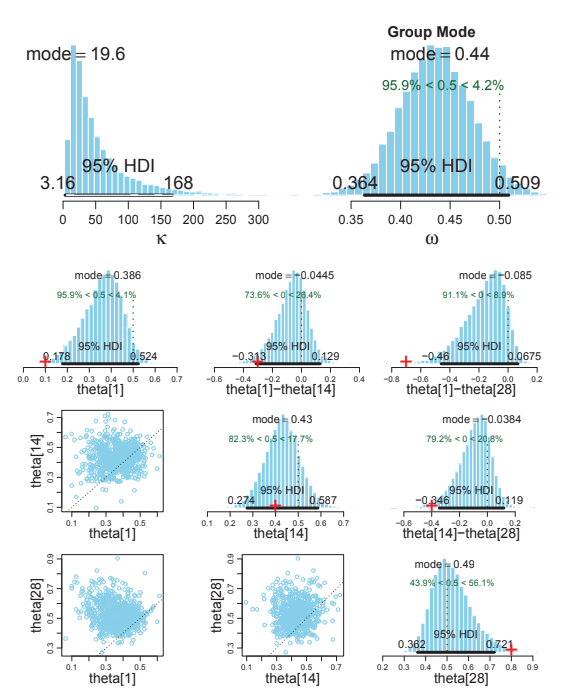
\includegraphics[width=\linewidth]{img/fig9_10}
\end{figure}
\end{columns}
\end{frame}

\begin{frame}
\frametitle{Priors in mid-level paramters}
\begin{columns}[c]
\column{.5\textwidth}
Priors (imputed from top-level priors) are sometimes unintended.

\vspace{1em}
In our case: Group mode prior is uniform. This results in uniform priors in $\theta$.

\vspace{1em}
Priors on differences: Difference between two uniform distributions (triangular).
\column{.5\textwidth}
\begin{figure}
\centering
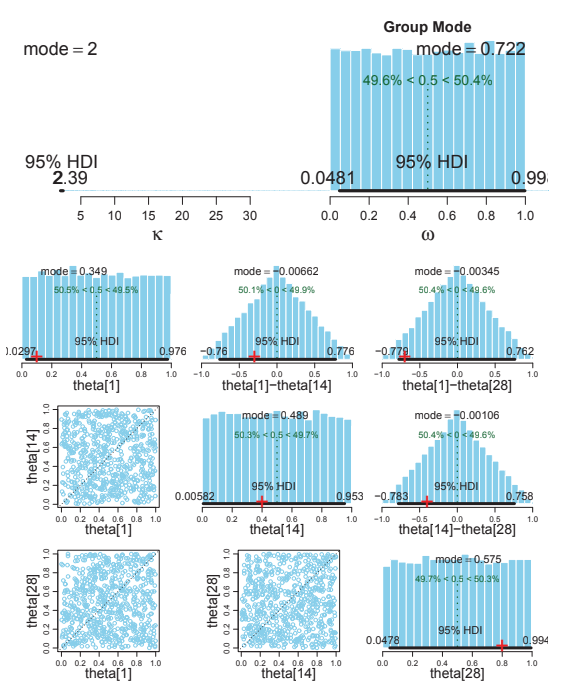
\includegraphics[width=\linewidth]{img/fig9_11}
\end{figure}
\end{columns}
\end{frame}

\begin{frame}
\frametitle{Shrinkage}
\begin{columns}[c]
\column{.5\textwidth}
Low level paramters cluster where high-level paramters are likely, called \emph{shrinkage}.

\vspace{1em}
In previous example: Estimates closer to group mode than sample mean.

\vspace{1em}
HL parameters influenced by all data. Low level, only by individual data. Property of hierarchical models.

\column{.5\textwidth}
\begin{figure}
\centering
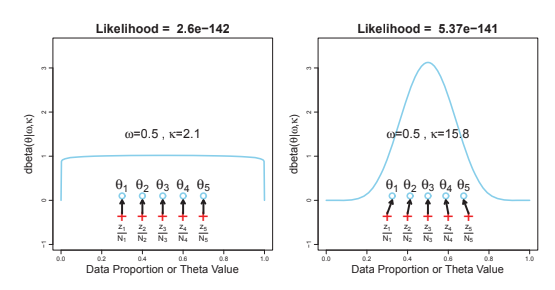
\includegraphics[width=\linewidth]{img/fig9_12}
\end{figure}
\end{columns}
\end{frame}

\begin{frame}
\begin{center}
{\huge{End!}}
\\\vspace{2em}
\end{center}
\end{frame}

\section{Appendix}
\begin{frame}
\frametitle{Aside: Efficiency vs. Effectiveness vs. Efficacy}
According to the Cambrigde Dictionary:
\begin{description}
\item[Efficiency] the good use of time and energy in a way that does not waste any
\item[Effectiveness] the ability to be successful and produce the intended results
\item[Efficacy] the ability, especially of a medicine or a method of achieving something, to produce the intended result (Am. E.: the quality of being effective; effectiveness)
\end{description}

\noindent\makebox[\linewidth]{\rule{0.95\textwidth}{0.4pt}}

\begin{description}
\item[Efficient] working or operating quickly and effectively in an organized way
\item[Effective] successful or achieving the results that you want
\item[Efficacious] able to produce the intended result 
\end{description}
\end{frame}

\begin{frame}
\begin{center}
{\huge{Remaining figures}}
\\\vspace{2em}
The rest of the chapter is mainly a more involved example, so figures are only included for discusion if necessary.
\end{center}
\end{frame}

\begin{frame}
\frametitle{Figure 9.13}
\begin{figure}
\centering
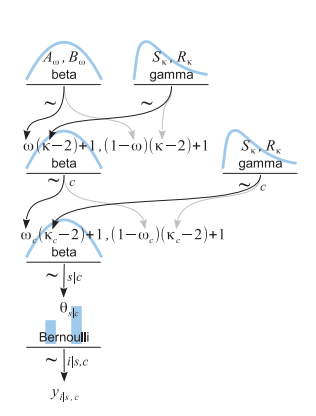
\includegraphics[height=0.8\textheight]{img/fig9_13}
\end{figure}

\end{frame}
\begin{frame}
\frametitle{Figure 9.14}
\begin{figure}
\centering
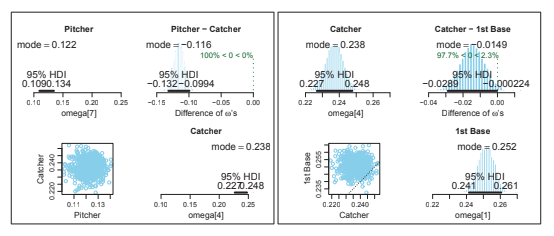
\includegraphics[width=\linewidth]{img/fig9_14}
\end{figure}
\end{frame}

\begin{frame}
\frametitle{Figure 9.15}
\begin{figure}
\centering
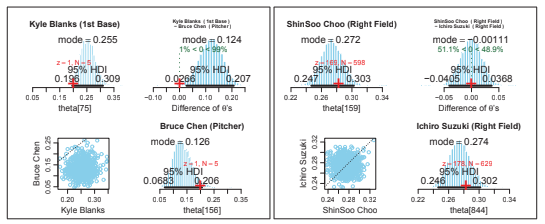
\includegraphics[width=\linewidth]{img/fig9_15}
\end{figure}
\end{frame}

\begin{frame}
\frametitle{Figure 9.16}
\begin{figure}
\centering
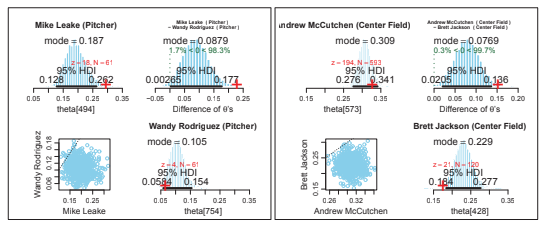
\includegraphics[width=\linewidth]{img/fig9_16}
\end{figure}
\end{frame}

\begin{frame}
\frametitle{Figure 9.17}
\begin{figure}
\centering
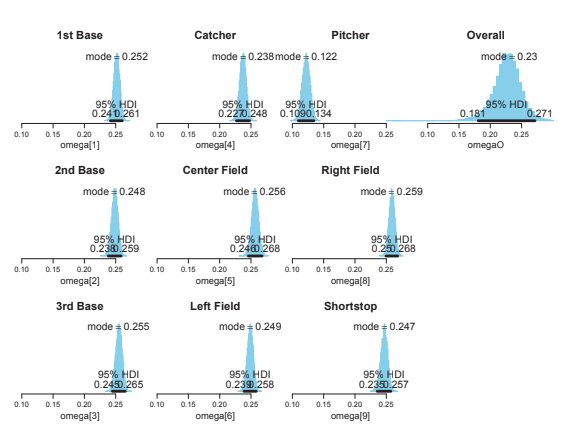
\includegraphics[height=0.8\textheight]{img/fig9_17}
\end{figure}
\end{frame}

\begin{frame}
\frametitle{Figure 9.18}
\begin{figure}
\centering
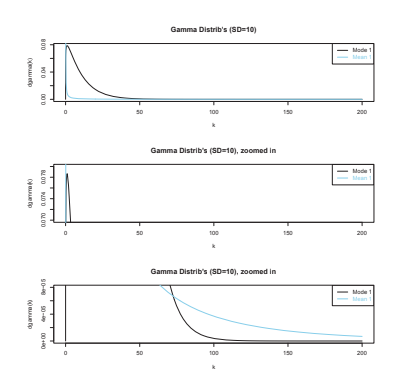
\includegraphics[height=0.8\textheight]{img/fig9_18}
\end{figure}
\end{frame}

\begin{frame}
\frametitle{Figure 9.19}
\begin{figure}
\centering
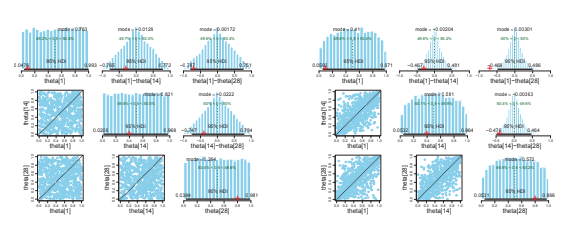
\includegraphics[width=\linewidth]{img/fig9_19}
\end{figure}
\end{frame}

\end{document} 